\section{Search\_\-Result  Class Reference}
\label{classSearch__Result}\index{Search_Result@{Search\_\-Result}}
{\tt \#include $<$dil2al.hh$>$}

Inheritance diagram for Search\_\-Result::\begin{figure}[H]
\begin{center}
\leavevmode
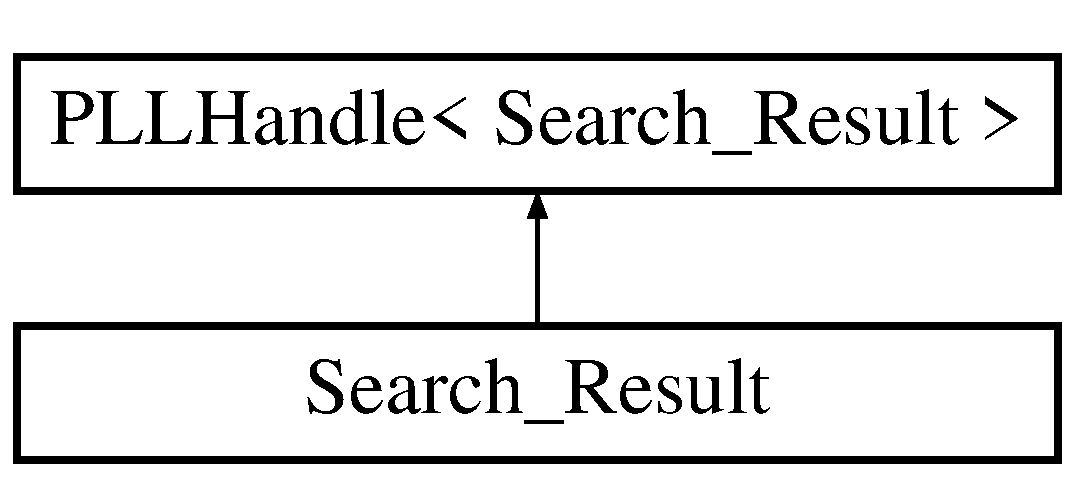
\includegraphics[height=2cm]{classSearch__Result}
\end{center}
\end{figure}
\subsection*{Public Types}
\begin{CompactItemize}
\item 
enum {\bf Search\_\-Result\_\-types} \{ {\bf SR\_\-REGULAR}, 
{\bf SR\_\-DIRECTORY\_\-ENTRY}, 
{\bf SR\_\-URL}
 \}
\end{CompactItemize}
\subsection*{Public Methods}
\begin{CompactItemize}
\item 
{\bf Search\_\-Result} (const char $\ast$s, const {\bf Target\_\-Access} \&t, {\bf String} \&text, const {\bf Big\-Regex} \&skrx)
\item 
{\bf Search\_\-Result\_\-types} {\bf Type} ()
\item 
int {\bf isequal} (const Search\_\-Result \&sr) const
\item 
int {\bf operator==} (const Search\_\-Result \&sr) const
\item 
int {\bf operator!=} (const Search\_\-Result \&sr) const
\item 
{\bf String} {\bf HTML\_\-put\_\-text} () const
\item 
{\bf operator const char $\ast$} () const
\end{CompactItemize}
\subsection*{Protected Attributes}
\begin{CompactItemize}
\item 
{\bf String} {\bf searchkey}
\item 
{\bf Target\_\-Access} {\bf target}
\item 
{\bf String} {\bf pretext}
\item 
{\bf String} {\bf keytext}
\item 
{\bf String} {\bf posttext}
\item 
long {\bf location}
\item 
{\bf Search\_\-Result\_\-types} {\bf type}
\end{CompactItemize}


\subsection{Member Enumeration Documentation}
\index{Search_Result@{Search\_\-Result}!Search_Result_types@{Search\_\-Result\_\-types}}
\index{Search_Result_types@{Search\_\-Result\_\-types}!Search_Result@{Search\_\-Result}}
\subsubsection{\setlength{\rightskip}{0pt plus 5cm}enum Search\_\-Result::Search\_\-Result\_\-types}\label{classSearch__Result_s3}


\begin{Desc}
\item[Enumeration values:]\par
\begin{description}
\index{SR_REGULAR@{SR\_\-REGULAR}!Search_Result@{Search\_\-Result}}\index{Search_Result@{Search\_\-Result}!SR_REGULAR@{SR\_\-REGULAR}}\item[{\em 
{\em SR\_\-REGULAR}\label{classSearch__Result_s3s0}
}]\index{SR_DIRECTORY_ENTRY@{SR\_\-DIRECTORY\_\-ENTRY}!Search_Result@{Search\_\-Result}}\index{Search_Result@{Search\_\-Result}!SR_DIRECTORY_ENTRY@{SR\_\-DIRECTORY\_\-ENTRY}}\item[{\em 
{\em SR\_\-DIRECTORY\_\-ENTRY}\label{classSearch__Result_s3s1}
}]\index{SR_URL@{SR\_\-URL}!Search_Result@{Search\_\-Result}}\index{Search_Result@{Search\_\-Result}!SR_URL@{SR\_\-URL}}\item[{\em 
{\em SR\_\-URL}\label{classSearch__Result_s3s2}
}]\end{description}
\end{Desc}



Definition at line 1052 of file dil2al.hh.

Referenced by Type().



\footnotesize\begin{verbatim}1052 { SR_REGULAR, SR_DIRECTORY_ENTRY, SR_URL };
\end{verbatim}\normalsize 


\subsection{Constructor \& Destructor Documentation}
\index{Search_Result@{Search\_\-Result}!Search_Result@{Search\_\-Result}}
\index{Search_Result@{Search\_\-Result}!Search_Result@{Search\_\-Result}}
\subsubsection{\setlength{\rightskip}{0pt plus 5cm}Search\_\-Result::Search\_\-Result (const char $\ast$ {\em s}, const {\bf Target\_\-Access} \& {\em t}, {\bf String} \& {\em text}, const {\bf Big\-Regex} \& {\em skrx})}\label{classSearch__Result_a0}




Definition at line 343 of file search.cc.

References String::at(), String::before(), String::contains(), String::from(), String::index(), keytext, String::length(), posttext, String::prepend(), pretext, String::SEARCH\_\-END, SR\_\-DIRECTORY\_\-ENTRY, SR\_\-REGULAR, String::sub(), Target\_\-Access::TA\_\-LOCAL\_\-DIRECTORY, type, and Target\_\-Access::Type().



\footnotesize\begin{verbatim}343                                                                                                          : searchkey(s), target(t), location(skrx.subpos()) {
344         // Obtains the matched keytext and some pretext and posttext
345         const int PTEXTSIZE = 160;
346         keytext = text.sub(skrx,0);
347         if (t.Type()!=Target_Access::TA_LOCAL_DIRECTORY) { // get pretext and posttext
348                 // *** DETECT HERE IF SR_URL!
349                 type = SR_REGULAR;
350                 if (skrx.subpos()>PTEXTSIZE) pretext = text.at(skrx.subpos()-PTEXTSIZE,PTEXTSIZE); else pretext = text.before(skrx.subpos());
351                 int skrxend = skrx.subpos()+skrx.sublen();
352                 if ((skrxend+PTEXTSIZE)<text.length()) posttext = text.at(skrxend,PTEXTSIZE); else posttext = text.from(skrxend);
353         } else { // get complete directory entry reference
354                 type = SR_DIRECTORY_ENTRY;
355                 int entrystart = text.index("<A HREF=",(int) (skrx.subpos()-text.length()));
356                 if (entrystart>=0) {
357                         int entryend = text.index("</A>",skrx.subpos());
358                         if (entryend>=0) {
359                                 int urlend = text.index("\">",String::SEARCH_END,entrystart);
360                                 if (urlend>=0) {
361                                         pretext = text.at(entrystart,urlend-entrystart); // get URL
362                                         // split reference text into pre, key and post parts
363                                         posttext = text.at(urlend,entryend-urlend);
364                                         if (posttext.contains(skrx)) {
365                                                 pretext += posttext.before(skrx.subpos());
366                                                 keytext = posttext.sub(skrx,0);
367                                                 posttext = posttext.from(skrx.subpos()+skrx.sublen());
368                                         } else { // should never occur in a SR_DIRECTORY_ENTRY, just for extra safety
369                                                 pretext += '[';
370                                                 posttext.prepend("] ");
371                                         }
372                                         posttext += "</A>";
373                                 }
374                         }
375                 }
376         }
377 }
\end{verbatim}\normalsize 


\subsection{Member Function Documentation}
\index{Search_Result@{Search\_\-Result}!HTML_put_text@{HTML\_\-put\_\-text}}
\index{HTML_put_text@{HTML\_\-put\_\-text}!Search_Result@{Search\_\-Result}}
\subsubsection{\setlength{\rightskip}{0pt plus 5cm}{\bf String} Search\_\-Result::HTML\_\-put\_\-text () const}\label{classSearch__Result_a5}




Definition at line 391 of file search.cc.

References HTML\_\-safe(), keytext, location, posttext, pretext, res, SR\_\-DIRECTORY\_\-ENTRY, SR\_\-REGULAR, SR\_\-URL, Target\_\-Access::Target(), and target.

Referenced by operator const char $\ast$().



\footnotesize\begin{verbatim}391                                           {
392         // Produce HTML output for search result
393         static String res;
394         String pre, post, key;
395         // *** IMPROVE:
396         // - identify any links in the pretext+keytext+posttext and turn them into correct relative links
397         // - beware of searchkey found in the middle of an HREF URL
398         switch (type) {
399                 case SR_REGULAR: // *** this one will be modified with the improvements mentioned above
400                         pre = pretext; key = keytext; post = posttext;
401                         res = "<A HREF=\""+target.Target()+"\">"+target.Target()+"</A> ["+String(location)+"]: "+(*HTML_safe(pre))+"<FONT COLOR=\"#FF0000\"><B>"+(*HTML_safe(key))+"</B></FONT>"+(*HTML_safe(post))+"\n<P>\n\n";
402                         break;
403                 case SR_DIRECTORY_ENTRY:
404                         res = "<A HREF=\""+target.Target()+"\">"+target.Target()+"</A>: "+pretext+"<FONT COLOR=\"#FF0000\"><B>"+keytext+"</B></FONT>"+posttext+"\n<P>\n\n";
405                         break;
406                 case SR_URL: // *** implement this correctly!
407                         res = "<A HREF=\""+target.Target()+"\">"+target.Target()+"</A> ["+String(location)+"]: "+pretext+"<FONT COLOR=\"#FF0000\"><B>"+keytext+"</B></FONT>"+posttext+"\n<P>\n\n";
408                         break;
409         }
410         return res;
411 }
\end{verbatim}\normalsize 
\index{Search_Result@{Search\_\-Result}!isequal@{isequal}}
\index{isequal@{isequal}!Search_Result@{Search\_\-Result}}
\subsubsection{\setlength{\rightskip}{0pt plus 5cm}int Search\_\-Result::isequal (const Search\_\-Result \& {\em sr}) const}\label{classSearch__Result_a2}




Definition at line 379 of file search.cc.

References keytext, posttext, pretext, searchkey, target, and type.

Referenced by operator!=(), and operator==().



\footnotesize\begin{verbatim}379                                                          {
380         // Equality comparison operator
381         // Note: This could also have been defined as a function that takes two arguments
382         if (searchkey!=sr.searchkey) return 0;
383         if (target!=sr.target) return 0;
384         if (pretext!=sr.pretext) return 0;
385         if (keytext!=sr.keytext) return 0;
386         if (posttext!=sr.posttext) return 0;
387         if (type!=sr.type) return 0;
388         return 1;
389 }
\end{verbatim}\normalsize 
\index{Search_Result@{Search\_\-Result}!operator const char *@{operator const char $\ast$}}
\index{operator const char *@{operator const char $\ast$}!Search_Result@{Search\_\-Result}}
\subsubsection{\setlength{\rightskip}{0pt plus 5cm}Search\_\-Result::operator const char $\ast$ () const\hspace{0.3cm}{\tt  [inline]}}\label{classSearch__Result_a6}




Definition at line 1069 of file dil2al.hh.

References HTML\_\-put\_\-text().



\footnotesize\begin{verbatim}1069 { return (const char *) HTML_put_text(); }
\end{verbatim}\normalsize 
\index{Search_Result@{Search\_\-Result}!operator"!=@{operator"!=}}
\index{operator"!=@{operator"!=}!Search_Result@{Search\_\-Result}}
\subsubsection{\setlength{\rightskip}{0pt plus 5cm}int Search\_\-Result::operator!= (const Search\_\-Result \& {\em sr}) const\hspace{0.3cm}{\tt  [inline]}}\label{classSearch__Result_a4}




Definition at line 1067 of file dil2al.hh.

References isequal().



\footnotesize\begin{verbatim}1067 { return (!isequal(sr)); }
\end{verbatim}\normalsize 
\index{Search_Result@{Search\_\-Result}!operator==@{operator==}}
\index{operator==@{operator==}!Search_Result@{Search\_\-Result}}
\subsubsection{\setlength{\rightskip}{0pt plus 5cm}int Search\_\-Result::operator== (const Search\_\-Result \& {\em sr}) const\hspace{0.3cm}{\tt  [inline]}}\label{classSearch__Result_a3}




Definition at line 1066 of file dil2al.hh.

References isequal().



\footnotesize\begin{verbatim}1066 { return isequal(sr); }
\end{verbatim}\normalsize 
\index{Search_Result@{Search\_\-Result}!Type@{Type}}
\index{Type@{Type}!Search_Result@{Search\_\-Result}}
\subsubsection{\setlength{\rightskip}{0pt plus 5cm}{\bf Search\_\-Result\_\-types} Search\_\-Result::Type ()\hspace{0.3cm}{\tt  [inline]}}\label{classSearch__Result_a1}




Definition at line 1064 of file dil2al.hh.

References Search\_\-Result\_\-types, and type.

Referenced by Search\_\-Target::search().



\footnotesize\begin{verbatim}1064 { return type; }
\end{verbatim}\normalsize 


\subsection{Member Data Documentation}
\index{Search_Result@{Search\_\-Result}!keytext@{keytext}}
\index{keytext@{keytext}!Search_Result@{Search\_\-Result}}
\subsubsection{\setlength{\rightskip}{0pt plus 5cm}{\bf String} Search\_\-Result::keytext\hspace{0.3cm}{\tt  [protected]}}\label{classSearch__Result_n3}




Definition at line 1057 of file dil2al.hh.

Referenced by HTML\_\-put\_\-text(), isequal(), and Search\_\-Result().\index{Search_Result@{Search\_\-Result}!location@{location}}
\index{location@{location}!Search_Result@{Search\_\-Result}}
\subsubsection{\setlength{\rightskip}{0pt plus 5cm}long Search\_\-Result::location\hspace{0.3cm}{\tt  [protected]}}\label{classSearch__Result_n5}




Definition at line 1058 of file dil2al.hh.

Referenced by HTML\_\-put\_\-text().\index{Search_Result@{Search\_\-Result}!posttext@{posttext}}
\index{posttext@{posttext}!Search_Result@{Search\_\-Result}}
\subsubsection{\setlength{\rightskip}{0pt plus 5cm}{\bf String} Search\_\-Result::posttext\hspace{0.3cm}{\tt  [protected]}}\label{classSearch__Result_n4}




Definition at line 1057 of file dil2al.hh.

Referenced by HTML\_\-put\_\-text(), isequal(), and Search\_\-Result().\index{Search_Result@{Search\_\-Result}!pretext@{pretext}}
\index{pretext@{pretext}!Search_Result@{Search\_\-Result}}
\subsubsection{\setlength{\rightskip}{0pt plus 5cm}{\bf String} Search\_\-Result::pretext\hspace{0.3cm}{\tt  [protected]}}\label{classSearch__Result_n2}




Definition at line 1057 of file dil2al.hh.

Referenced by HTML\_\-put\_\-text(), isequal(), and Search\_\-Result().\index{Search_Result@{Search\_\-Result}!searchkey@{searchkey}}
\index{searchkey@{searchkey}!Search_Result@{Search\_\-Result}}
\subsubsection{\setlength{\rightskip}{0pt plus 5cm}{\bf String} Search\_\-Result::searchkey\hspace{0.3cm}{\tt  [protected]}}\label{classSearch__Result_n0}




Definition at line 1055 of file dil2al.hh.

Referenced by isequal().\index{Search_Result@{Search\_\-Result}!target@{target}}
\index{target@{target}!Search_Result@{Search\_\-Result}}
\subsubsection{\setlength{\rightskip}{0pt plus 5cm}{\bf Target\_\-Access} Search\_\-Result::target\hspace{0.3cm}{\tt  [protected]}}\label{classSearch__Result_n1}




Definition at line 1056 of file dil2al.hh.

Referenced by HTML\_\-put\_\-text(), and isequal().\index{Search_Result@{Search\_\-Result}!type@{type}}
\index{type@{type}!Search_Result@{Search\_\-Result}}
\subsubsection{\setlength{\rightskip}{0pt plus 5cm}{\bf Search\_\-Result\_\-types} Search\_\-Result::type\hspace{0.3cm}{\tt  [protected]}}\label{classSearch__Result_n6}




Definition at line 1059 of file dil2al.hh.

Referenced by isequal(), Search\_\-Result(), and Type().

The documentation for this class was generated from the following files:\begin{CompactItemize}
\item 
{\bf dil2al.hh}\item 
{\bf search.cc}\end{CompactItemize}
